\documentclass[11pt]{article}
\usepackage[margin=1in]{geometry}
\usepackage{booktabs}
\usepackage{amsmath}
\usepackage{amssymb}
\usepackage{graphicx}
\usepackage{xcolor}
\usepackage{caption}
\usepackage{capt-of}
\usepackage{tikz}
\usetikzlibrary{arrows.meta}
\title{LoCoBench: Logical Coherence Score Evaluation\\
\large The gold-relation arm on generated items}
\author{FactReasoner --- LoCoBench evaluation}
\date{\today}


\begin{document}

\maketitle

\section{Setup}

This report evaluates the Logical Coherence Score (LCS) pipeline on the \textbf{10 generated items} of \texttt{locobench-claude-5-fixed}. Unlike the mining experiments, relations are \emph{not} mined by a model here: each item already carries its inter-atom relations as gold labels, and those labels are compiled directly into the coherence MRF. No LLM is involved, so every number below is deterministic and reproducible offline (Merlin is the only subprocess).

\paragraph{Atom priors.} An atom's unary factor is $[1-\pi_i, \pi_i]$ with $\pi_i = 0.9$ when the item marks the atom \texttt{factual} and $\pi_i = 0.1$ when it does not. The coherence MRF therefore starts from the corpus's own factuality labels --- the label-driven analogue of the two-stage model, where stage~1's posterior marginals play this role. Hard $1/0$ priors are deliberately avoided: they would zero out worlds and make several readouts degenerate.

\paragraph{Edge probabilities.} A gold relation carries an intended strength band and a strength range; the factor probability is the range's \textbf{midpoint} (strong $[0.85,1] \to 0.925$, moderate $[0.6,0.84] \to 0.720$, weak $[0.35,0.59] \to 0.470$). Because gold is a \emph{label} rather than an estimate, the type confidence $P(\tau \mid a_i,a_j)$ is fixed at $1.0$ and the conditional strength is that same midpoint. Any apparent precision beyond the band is an artefact of the midpoint convention, not a measurement.

\paragraph{Resolved concessions.} A concession the text resolves is softened by $p \mapsto p\,(1-\lambda)$ with $\lambda = 0.45$ (deep-dive Eq.~2). The resolver is read from the item's own \texttt{resolver\_atom\_id}, so the miner's text heuristic for spotting a holding atom is bypassed entirely --- when the label states the resolver, guessing it would be the wrong instrument.

\paragraph{Ordering-only relations.} \texttt{Precedence} and \texttt{Succession} compile to Level-1 \texttt{none}: they record source/target order but couple no truth values, so they contribute \textbf{no factor}. They are counted in the dataset table and excluded from the MRF, exactly as \texttt{lcs.taxonomy.compile\_sense} dictates.

\paragraph{Arms.} Each item is scored under \textbf{\texttt{gold}} (all gold edges) and \textbf{\texttt{gold\_valid}} (valid edges only). The second arm drops the deliberately-planted invalid relations, which isolates what those planted errors cost. All four readouts are computed for both: \texttt{mean\_marginal}, \texttt{consistency}, \texttt{reified}, \texttt{log\_partition}.

\section{Dataset}

\begin{table}[htbp]
\centering
\small
\caption{Per-item size. \textbf{Gold} is every relation the item lists; \textbf{ord-only} are the Precedence/Succession edges that carry no truth coupling and so produce no factor; \textbf{MRF} is what remains and is scored; \textbf{valid} is the subset whose \texttt{validity} is \texttt{valid}.}
\label{tab:dataset}
\begin{tabular}{lllrrrrr}
\toprule
Family & Rung & Name & Atoms & Gold & ord-only & MRF & valid \\
\midrule
\texttt{f001} & 0 & worse & 16 & 11 & 1 & 10 & 5 \\
\texttt{f001} & 1 & base & 16 & 10 & 1 & 9 & 5 \\
\texttt{f001} & 2 & concession\_resolved & 16 & 10 & 1 & 9 & 5 \\
\texttt{f001} & 3 & fix\_one\_conflict & 16 & 9 & 1 & 8 & 5 \\
\texttt{f001} & 4 & coherent & 16 & 8 & 1 & 7 & 4 \\
\texttt{f002} & 0 & worse & 16 & 11 & 1 & 10 & 6 \\
\texttt{f002} & 1 & base & 16 & 10 & 1 & 9 & 6 \\
\texttt{f002} & 2 & concession\_resolved & 16 & 10 & 1 & 9 & 6 \\
\texttt{f002} & 3 & fix\_one\_conflict & 16 & 9 & 1 & 8 & 6 \\
\texttt{f002} & 4 & coherent & 16 & 8 & 1 & 7 & 6 \\
\bottomrule
\end{tabular}
\end{table}

Across the dataset there are 160 atoms, of which 140 are marked \texttt{factual} (prior 0.9) and 20 are not (prior 0.1).

\begin{minipage}[t]{0.48\linewidth}
\centering
\small
\captionof{table}{Level-2 discourse senses.}
\label{tab:senses}
\begin{tabular}{lr}
\toprule
Value & Count \\
\midrule
\texttt{Contrast} & 17 \\
\texttt{Evidence} & 15 \\
\texttt{Cause-Effect} & 10 \\
\texttt{Concession} & 10 \\
\texttt{Disjunction} & 10 \\
\texttt{Precedence} & 10 \\
\texttt{Restatement} & 10 \\
\texttt{Alternative} & 9 \\
\texttt{Effect-Cause} & 5 \\
\bottomrule
\end{tabular}
\end{minipage}\hfill\begin{minipage}[t]{0.48\linewidth}
\centering
\small
\captionof{table}{Level-1 couplings.}
\label{tab:couplings}
\begin{tabular}{lr}
\toprule
Value & Count \\
\midrule
\texttt{entailment} & 30 \\
\texttt{contradiction} & 27 \\
\texttt{co\_necessity} & 10 \\
\texttt{equivalence} & 10 \\
\texttt{none} & 10 \\
\texttt{exclusive} & 9 \\
\bottomrule
\end{tabular}
\end{minipage}

\bigskip
\begin{minipage}[t]{0.48\linewidth}
\centering
\small
\captionof{table}{Relation validity.}
\label{tab:validity}
\begin{tabular}{lr}
\toprule
Value & Count \\
\midrule
\texttt{valid} & 59 \\
\texttt{invalid} & 37 \\
\bottomrule
\end{tabular}
\end{minipage}\hfill\begin{minipage}[t]{0.48\linewidth}
\centering
\small
\captionof{table}{Planted error kinds.}
\label{tab:errorkinds}
\begin{tabular}{lr}
\toprule
Value & Count \\
\midrule
\texttt{spurious} & 12 \\
\texttt{false\_endpoint} & 10 \\
\texttt{wrong\_direction} & 10 \\
\texttt{wrong\_sense} & 5 \\
\bottomrule
\end{tabular}
\end{minipage}

\noindent 37 of 96 gold relations (39\%) are deliberately invalid: the corpus plants relation-level errors so a system's ability to \emph{recover} the intended graph can be graded. The \texttt{gold} arm scores the graph as labelled, including those errors; the \texttt{gold\_valid} arm scores only the intended-correct subgraph.

\section{LCS scores}

\begin{table}[htbp]
\centering
\small
\caption{LCS readouts, arm \texttt{gold} (all gold edges). Higher is more coherent for every readout. \textbf{Rel} is the number of edge-producing relations in the MRF.}
\label{tab:scores-gold}
\begin{tabular}{llrrrrrr}
\toprule
Family & Rung & Rel & \textbf{mean-marg} & \textbf{consist} & \textbf{reified} & \textbf{log-Z} & $\log Z$ \\
\midrule
\texttt{f001} & 0 (worse) & 10 & 0.750 & 0.131 & 0.151 & 0.343 & -8.01 \\
\texttt{f001} & 1 (base) & 9 & 0.761 & 0.341 & 0.222 & 0.375 & -6.93 \\
\texttt{f001} & 2 (concession\_resolved) & 9 & 0.790 & 0.085 & 0.253 & 0.374 & -5.75 \\
\texttt{f001} & 3 (fix\_one\_conflict) & 8 & 0.789 & 0.094 & 0.262 & 0.425 & -5.07 \\
\texttt{f001} & 4 (coherent) & 7 & 0.823 & 0.128 & 0.321 & 0.489 & -3.59 \\
\midrule
\texttt{f002} & 0 (worse) & 10 & 0.786 & 0.016 & 0.120 & 0.281 & -7.05 \\
\texttt{f002} & 1 (base) & 9 & 0.792 & 0.075 & 0.250 & 0.327 & -5.88 \\
\texttt{f002} & 2 (concession\_resolved) & 9 & 0.824 & 0.015 & 0.240 & 0.325 & -4.84 \\
\texttt{f002} & 3 (fix\_one\_conflict) & 8 & 0.824 & 0.016 & 0.248 & 0.393 & -4.15 \\
\texttt{f002} & 4 (coherent) & 7 & 0.824 & 0.018 & 0.257 & 0.500 & -3.46 \\
\bottomrule
\end{tabular}
\end{table}

\begin{table}[htbp]
\centering
\small
\caption{LCS readouts, arm \texttt{gold\_valid} (valid edges only). Higher is more coherent for every readout. \textbf{Rel} is the number of edge-producing relations in the MRF.}
\label{tab:scores-gold-valid}
\begin{tabular}{llrrrrrr}
\toprule
Family & Rung & Rel & \textbf{mean-marg} & \textbf{consist} & \textbf{reified} & \textbf{log-Z} & $\log Z$ \\
\midrule
\texttt{f001} & 0 (worse) & 5 & 0.749 & 0.450 & 0.334 & 0.432 & -4.45 \\
\texttt{f001} & 1 (base) & 5 & 0.749 & 0.450 & 0.334 & 0.432 & -4.45 \\
\texttt{f001} & 2 (concession\_resolved) & 5 & 0.781 & 0.127 & 0.294 & 0.441 & -3.51 \\
\texttt{f001} & 3 (fix\_one\_conflict) & 5 & 0.781 & 0.127 & 0.294 & 0.441 & -3.51 \\
\texttt{f001} & 4 (coherent) & 4 & 0.814 & 0.173 & 0.357 & 0.514 & -2.03 \\
\midrule
\texttt{f002} & 0 (worse) & 6 & 0.792 & 0.092 & 0.269 & 0.435 & -3.76 \\
\texttt{f002} & 1 (base) & 6 & 0.792 & 0.092 & 0.269 & 0.435 & -3.76 \\
\texttt{f002} & 2 (concession\_resolved) & 6 & 0.824 & 0.018 & 0.258 & 0.498 & -2.71 \\
\texttt{f002} & 3 (fix\_one\_conflict) & 6 & 0.824 & 0.018 & 0.258 & 0.498 & -2.71 \\
\texttt{f002} & 4 (coherent) & 6 & 0.824 & 0.018 & 0.258 & 0.498 & -2.71 \\
\bottomrule
\end{tabular}
\end{table}

\subsection{Effect of the planted invalid relations}

Removing the deliberately-invalid gold relations is the clearest single-number effect in this evaluation. The planted errors are predominantly conflict edges attached to a false endpoint, so deleting them removes active contradictions: the conflict-sensitive readouts move sharply, while \texttt{mean\_marginal} --- an average over atom marginals already pinned near their $0.9/0.1$ priors --- barely moves.

\begin{table}[htbp]
\centering
\small
\caption{Change in each readout from arm \texttt{gold} to arm \texttt{gold\_valid} (valid edges only). Positive means the intended-correct subgraph scores as more coherent.}
\label{tab:arm-delta}
\begin{tabular}{llrrrrr}
\toprule
Family & Rung & Rel & \textbf{mean-marg} & \textbf{consist} & \textbf{reified} & \textbf{log-Z} \\
\midrule
\texttt{f001} & 0 & 10 $\to$ 5 & -0.001 & +0.318 & +0.183 & +0.090 \\
\texttt{f001} & 1 & 9 $\to$ 5 & -0.011 & +0.109 & +0.112 & +0.058 \\
\texttt{f001} & 2 & 9 $\to$ 5 & -0.009 & +0.042 & +0.041 & +0.067 \\
\texttt{f001} & 3 & 8 $\to$ 5 & -0.008 & +0.033 & +0.032 & +0.016 \\
\texttt{f001} & 4 & 7 $\to$ 4 & -0.008 & +0.046 & +0.036 & +0.026 \\
\texttt{f002} & 0 & 10 $\to$ 6 & +0.007 & +0.076 & +0.149 & +0.153 \\
\texttt{f002} & 1 & 9 $\to$ 6 & -0.000 & +0.017 & +0.019 & +0.107 \\
\texttt{f002} & 2 & 9 $\to$ 6 & -0.000 & +0.003 & +0.019 & +0.173 \\
\texttt{f002} & 3 & 8 $\to$ 6 & +0.000 & +0.002 & +0.010 & +0.105 \\
\texttt{f002} & 4 & 7 $\to$ 6 & +0.001 & +0.000 & +0.001 & -0.002 \\
\bottomrule
\end{tabular}
\end{table}

\section{Ladder ordering constraints}\label{sec:ladder}

Each family declares the ordering its rungs are meant to exhibit; the graded readouts are \texttt{mean\_marginal}, \texttt{consistency}, \texttt{log\_partition}.

\paragraph{Every rung carries its own gold relations.} In each family the five rungs carry \emph{different} gold relation sets, so each rung's labels describe the response that ships with them and the ordering constraints below are a genuine test of the readouts rather than a measurement of the corpus. This is what the per-rung relation transforms in \texttt{locobench.perturb} (\texttt{apply\_calls} / \texttt{plan\_targets}) provide: a rung's edges are the base edge set with that rung's own perturbations applied, each call targeting a distinct eligible edge, and a rung whose edge set still matches its parent's while its calls claim a change is rejected at generation time.

\paragraph{Read the two arms differently.} A \texttt{fix\_one\_conflict} or \texttt{coherent} rung removes the \emph{planted-invalid} conflicts first --- those are the edges a fix most plausibly deletes. The \texttt{gold\_valid} arm has already discarded exactly those edges, so consecutive rungs can share an identical valid subgraph and that arm is close to flat by construction. Its strict-increase failures are therefore expected and carry no information about the readouts; \textbf{the \texttt{gold} arm is the one the ladder constraints are about}. The valid-only arm remains useful for what it was added for: quantifying what the planted errors cost at a fixed rung.

\subsection*{Family \texttt{f001} (Anthropology, CONFLICT)}

Gold relations identical across rungs: \textbf{no}; distinct response texts: 5 of 5.

\begin{table}[htbp]
\centering
\small
\caption{Ordering constraints for \texttt{f001}, arm \texttt{gold}: 11 of 14 hold. C1 asserts a strict increase; C2 asserts a predicted decrease or invariance; C3 asserts endpoint separation.}
\label{tab:ladder-f001-gold}
\begin{tabular}{lllllrc}
\toprule
Class & Readout & Rungs & Expected & Observed & $\Delta$ & OK \\
\midrule
\texttt{C1} & \texttt{mean-marg} & 0$\to$1 & increase & increase & 0.010 & \checkmark \\
\texttt{C1} & \texttt{consist} & 0$\to$1 & increase & increase & 0.209 & \checkmark \\
\texttt{C1} & \texttt{log-Z} & 0$\to$1 & increase & increase & 0.032 & \checkmark \\
\texttt{C1} & \texttt{mean-marg} & 1$\to$2 & increase & increase & 0.029 & \checkmark \\
\texttt{C1} & \texttt{mean-marg} & 2$\to$3 & increase & decrease & -0.000 & $\times$ \\
\texttt{C1} & \texttt{log-Z} & 2$\to$3 & increase & increase & 0.051 & \checkmark \\
\texttt{C1} & \texttt{mean-marg} & 3$\to$4 & increase & increase & 0.034 & \checkmark \\
\texttt{C1} & \texttt{consist} & 3$\to$4 & increase & increase & 0.034 & \checkmark \\
\texttt{C1} & \texttt{log-Z} & 3$\to$4 & increase & increase & 0.063 & \checkmark \\
\texttt{C2} & \texttt{consist} & 1$\to$2 & decrease & decrease & -0.256 & \checkmark \\
\texttt{C2} & \texttt{log-Z} & 1$\to$2 & invariant & decrease & -0.000 & $\times$ \\
\texttt{C3} & \texttt{mean-marg} & 0$\to$4 & increase & increase & 0.072 & \checkmark \\
\texttt{C3} & \texttt{consist} & 0$\to$4 & increase & decrease & -0.004 & $\times$ \\
\texttt{C3} & \texttt{log-Z} & 0$\to$4 & increase & increase & 0.146 & \checkmark \\
\bottomrule
\end{tabular}
\end{table}

\begin{table}[htbp]
\centering
\small
\caption{Ordering constraints for \texttt{f001}, arm \texttt{gold\_valid}: 7 of 14 hold. C1 asserts a strict increase; C2 asserts a predicted decrease or invariance; C3 asserts endpoint separation.}
\label{tab:ladder-f001-gold-valid}
\begin{tabular}{lllllrc}
\toprule
Class & Readout & Rungs & Expected & Observed & $\Delta$ & OK \\
\midrule
\texttt{C1} & \texttt{mean-marg} & 0$\to$1 & increase & invariant & 0.000 & $\times$ \\
\texttt{C1} & \texttt{consist} & 0$\to$1 & increase & invariant & 0.000 & $\times$ \\
\texttt{C1} & \texttt{log-Z} & 0$\to$1 & increase & invariant & 0.000 & $\times$ \\
\texttt{C1} & \texttt{mean-marg} & 1$\to$2 & increase & increase & 0.032 & \checkmark \\
\texttt{C1} & \texttt{mean-marg} & 2$\to$3 & increase & invariant & 0.000 & $\times$ \\
\texttt{C1} & \texttt{log-Z} & 2$\to$3 & increase & invariant & 0.000 & $\times$ \\
\texttt{C1} & \texttt{mean-marg} & 3$\to$4 & increase & increase & 0.034 & \checkmark \\
\texttt{C1} & \texttt{consist} & 3$\to$4 & increase & increase & 0.046 & \checkmark \\
\texttt{C1} & \texttt{log-Z} & 3$\to$4 & increase & increase & 0.073 & \checkmark \\
\texttt{C2} & \texttt{consist} & 1$\to$2 & decrease & decrease & -0.323 & \checkmark \\
\texttt{C2} & \texttt{log-Z} & 1$\to$2 & invariant & increase & 0.009 & $\times$ \\
\texttt{C3} & \texttt{mean-marg} & 0$\to$4 & increase & increase & 0.065 & \checkmark \\
\texttt{C3} & \texttt{consist} & 0$\to$4 & increase & decrease & -0.277 & $\times$ \\
\texttt{C3} & \texttt{log-Z} & 0$\to$4 & increase & increase & 0.082 & \checkmark \\
\bottomrule
\end{tabular}
\end{table}

\subsection*{Family \texttt{f002} (Archaeology, CONFLICT)}

Gold relations identical across rungs: \textbf{no}; distinct response texts: 5 of 5.

\begin{table}[htbp]
\centering
\small
\caption{Ordering constraints for \texttt{f002}, arm \texttt{gold}: 11 of 14 hold. C1 asserts a strict increase; C2 asserts a predicted decrease or invariance; C3 asserts endpoint separation.}
\label{tab:ladder-f002-gold}
\begin{tabular}{lllllrc}
\toprule
Class & Readout & Rungs & Expected & Observed & $\Delta$ & OK \\
\midrule
\texttt{C1} & \texttt{mean-marg} & 0$\to$1 & increase & increase & 0.007 & \checkmark \\
\texttt{C1} & \texttt{consist} & 0$\to$1 & increase & increase & 0.059 & \checkmark \\
\texttt{C1} & \texttt{log-Z} & 0$\to$1 & increase & increase & 0.046 & \checkmark \\
\texttt{C1} & \texttt{mean-marg} & 1$\to$2 & increase & increase & 0.032 & \checkmark \\
\texttt{C1} & \texttt{mean-marg} & 2$\to$3 & increase & decrease & -0.000 & $\times$ \\
\texttt{C1} & \texttt{log-Z} & 2$\to$3 & increase & increase & 0.069 & \checkmark \\
\texttt{C1} & \texttt{mean-marg} & 3$\to$4 & increase & decrease & -0.000 & $\times$ \\
\texttt{C1} & \texttt{consist} & 3$\to$4 & increase & increase & 0.002 & \checkmark \\
\texttt{C1} & \texttt{log-Z} & 3$\to$4 & increase & increase & 0.106 & \checkmark \\
\texttt{C2} & \texttt{consist} & 1$\to$2 & decrease & decrease & -0.061 & \checkmark \\
\texttt{C2} & \texttt{log-Z} & 1$\to$2 & invariant & decrease & -0.002 & $\times$ \\
\texttt{C3} & \texttt{mean-marg} & 0$\to$4 & increase & increase & 0.038 & \checkmark \\
\texttt{C3} & \texttt{consist} & 0$\to$4 & increase & increase & 0.002 & \checkmark \\
\texttt{C3} & \texttt{log-Z} & 0$\to$4 & increase & increase & 0.218 & \checkmark \\
\bottomrule
\end{tabular}
\end{table}

\begin{table}[htbp]
\centering
\small
\caption{Ordering constraints for \texttt{f002}, arm \texttt{gold\_valid}: 4 of 14 hold. C1 asserts a strict increase; C2 asserts a predicted decrease or invariance; C3 asserts endpoint separation.}
\label{tab:ladder-f002-gold-valid}
\begin{tabular}{lllllrc}
\toprule
Class & Readout & Rungs & Expected & Observed & $\Delta$ & OK \\
\midrule
\texttt{C1} & \texttt{mean-marg} & 0$\to$1 & increase & invariant & 0.000 & $\times$ \\
\texttt{C1} & \texttt{consist} & 0$\to$1 & increase & invariant & 0.000 & $\times$ \\
\texttt{C1} & \texttt{log-Z} & 0$\to$1 & increase & invariant & 0.000 & $\times$ \\
\texttt{C1} & \texttt{mean-marg} & 1$\to$2 & increase & increase & 0.032 & \checkmark \\
\texttt{C1} & \texttt{mean-marg} & 2$\to$3 & increase & invariant & 0.000 & $\times$ \\
\texttt{C1} & \texttt{log-Z} & 2$\to$3 & increase & invariant & 0.000 & $\times$ \\
\texttt{C1} & \texttt{mean-marg} & 3$\to$4 & increase & invariant & 0.000 & $\times$ \\
\texttt{C1} & \texttt{consist} & 3$\to$4 & increase & invariant & 0.000 & $\times$ \\
\texttt{C1} & \texttt{log-Z} & 3$\to$4 & increase & invariant & 0.000 & $\times$ \\
\texttt{C2} & \texttt{consist} & 1$\to$2 & decrease & decrease & -0.074 & \checkmark \\
\texttt{C2} & \texttt{log-Z} & 1$\to$2 & invariant & increase & 0.063 & $\times$ \\
\texttt{C3} & \texttt{mean-marg} & 0$\to$4 & increase & increase & 0.032 & \checkmark \\
\texttt{C3} & \texttt{consist} & 0$\to$4 & increase & decrease & -0.074 & $\times$ \\
\texttt{C3} & \texttt{log-Z} & 0$\to$4 & increase & increase & 0.063 & \checkmark \\
\bottomrule
\end{tabular}
\end{table}

\section{Worked examples}

Each example gives the response as generated, its atoms with the priors their \texttt{factual} labels induce, the relation graph the gold labels build, and the specific relations with the factor probability each contributed.

\subsection{Anthropology -- base (\texttt{locobench-claude-5-fixed-f001-r1})}

\textbf{Topic:} Anthropology (Social Sciences). \textbf{Family:} \texttt{f001} (CONFLICT), rung 1 (\emph{base}). \textbf{Scores:} mean-marg $= 0.761$, consist $= 0.341$, reified $= 0.222$, log-Z $= 0.375$.



\paragraph{Framing question.} \emph{How do anthropologists adjudicate between rival interpretations when skeletal remains at a burial site show signs of trauma, and what evidence establishes whether the injuries were inflicted by human violence or by post-mortem processes?}



\paragraph{Response.} {\small Adjudication between rival readings of a traumatized skeleton begins as a matter of procedure rather than interpretation, because the evidentiary value of a lesion depends on how much is known about its context. Excavators record the position and orientation of each bone in situ before the remains are lifted, and only once that mapping is complete do several independent osteologists score the same lesions to test inter-observer reliability. Ordering the work in this way ensures that the descriptive record is fixed while the burial is still articulated, and that the scoring of margins, depressions and fracture surfaces can later be checked against a documented spatial arrangement rather than against the recollection of whoever first noticed the damage.

The analytical leverage in such disputes comes from the mechanics of bone itself, which change as the tissue's organic fraction degrades. The loss of collagen after death shifts the bone's response to loading from plastic to brittle, so that the same blow yields quite different failure geometry depending on when it was delivered. By contrast, buried bone retains its fresh, plastic mechanical properties for approximately fifty years after death, a durability that determines how wide the diagnostic window for early damage can reasonably be drawn.

Those material states leave characteristic signatures on the break surface, and it is these that carry most of the interpretive weight. Perimortem fractures in fresh bone produce beveled or obliquely angled fracture margins, whereas postmortem breaks in dry bone typically show transverse edges meeting the cortical surface at right angles; indeed, the plastic-to-brittle shift in loading response noted above is itself a consequence of that right-angled transverse geometry. The picture is complicated by the fact that postmortem dry-bone fractures produce beveled margins with adhering flakes of cortical bone. Even so, adhering bone flakes and hinge fractures indicate the bone was fresh when it broke, and analysts continue to treat that combination as the most reliable single criterion available to them.

Applied to a contested specimen, the reasoning runs from timing to morphology. The fracture occurred while the bone was still fresh and elastic, which confirms that flaking and hinging are markers of fresh-bone breakage; in other words, the break happened at or near the time of death, before the bone's collagen degraded. At the level of the whole assemblage, the dispute reduces to two mutually exclusive readings, exactly one of which must be right: either every fracture margin on the skeleton was produced after death, or at least one fracture margin on the skeleton was produced at or around the time of death. Faced with precisely this choice in the case at hand, the review panel ultimately held that beveled fracture margins on the cranium reflect perimortem breakage, a determination that dissolved the apparent conflict between the two accounts of beveling by fixing which of them governs the cranial evidence.

Establishing that a break is early does not by itself establish human violence, since several agencies operate on a body in the ground and each leaves its own configuration of displacement and damage. Ranking those agencies against the field documentation is the final step. For this assemblage, at least one of two processes was at work, and perhaps both: scavenging animals disturbed the remains within the grave, or sediment loading fractured the bones after burial. Distinguishing them relies on the recorded orientation of elements, the distribution of tooth pitting and the compression geometry of the affected shafts. A further source of confusion arises from the recovery process itself, for damage inflicted by trowels and picks during excavation can mimic ancient trauma; such tool damage is what caused the post-burial fracturing under sediment load in these bones, and its recognition is therefore a precondition of any claim about interpersonal violence.}

\begin{figure}[htbp]
\centering
\begin{minipage}[t]{0.48\linewidth}\centering
\resizebox{!}{6.4cm}{%
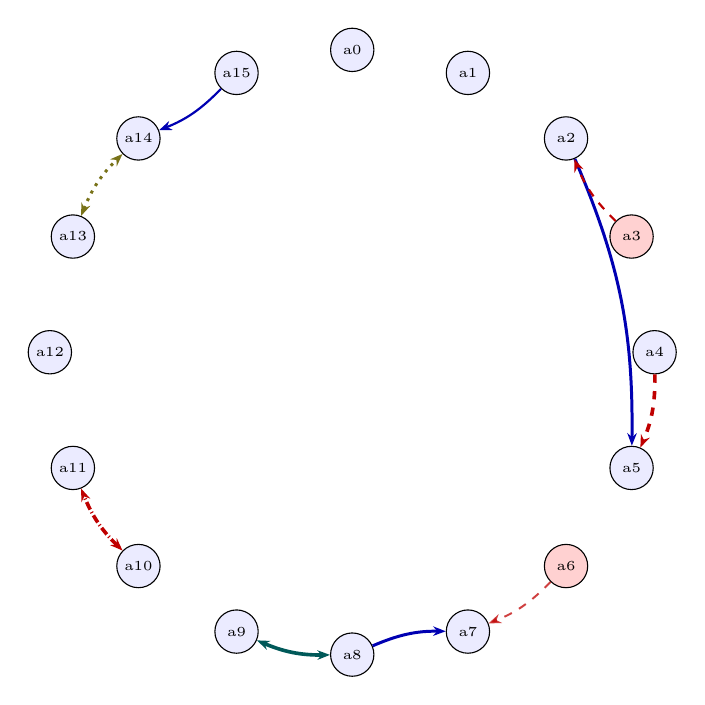
\begin{tikzpicture}[>={Stealth[length=1.6mm]}]
  \node[circle,draw,fill=blue!8,inner sep=1pt,minimum size=5.5mm,font=\tiny] (a0) at (90.0:3.84) {a0};
  \node[circle,draw,fill=blue!8,inner sep=1pt,minimum size=5.5mm,font=\tiny] (a1) at (67.5:3.84) {a1};
  \node[circle,draw,fill=blue!8,inner sep=1pt,minimum size=5.5mm,font=\tiny] (a2) at (45.0:3.84) {a2};
  \node[circle,draw,fill=red!18,inner sep=1pt,minimum size=5.5mm,font=\tiny] (a3) at (22.5:3.84) {a3};
  \node[circle,draw,fill=blue!8,inner sep=1pt,minimum size=5.5mm,font=\tiny] (a4) at (0.0:3.84) {a4};
  \node[circle,draw,fill=blue!8,inner sep=1pt,minimum size=5.5mm,font=\tiny] (a5) at (-22.5:3.84) {a5};
  \node[circle,draw,fill=red!18,inner sep=1pt,minimum size=5.5mm,font=\tiny] (a6) at (-45.0:3.84) {a6};
  \node[circle,draw,fill=blue!8,inner sep=1pt,minimum size=5.5mm,font=\tiny] (a7) at (-67.5:3.84) {a7};
  \node[circle,draw,fill=blue!8,inner sep=1pt,minimum size=5.5mm,font=\tiny] (a8) at (-90.0:3.84) {a8};
  \node[circle,draw,fill=blue!8,inner sep=1pt,minimum size=5.5mm,font=\tiny] (a9) at (-112.5:3.84) {a9};
  \node[circle,draw,fill=blue!8,inner sep=1pt,minimum size=5.5mm,font=\tiny] (a10) at (-135.0:3.84) {a10};
  \node[circle,draw,fill=blue!8,inner sep=1pt,minimum size=5.5mm,font=\tiny] (a11) at (-157.5:3.84) {a11};
  \node[circle,draw,fill=blue!8,inner sep=1pt,minimum size=5.5mm,font=\tiny] (a12) at (-180.0:3.84) {a12};
  \node[circle,draw,fill=blue!8,inner sep=1pt,minimum size=5.5mm,font=\tiny] (a13) at (-202.5:3.84) {a13};
  \node[circle,draw,fill=blue!8,inner sep=1pt,minimum size=5.5mm,font=\tiny] (a14) at (-225.0:3.84) {a14};
  \node[circle,draw,fill=blue!8,inner sep=1pt,minimum size=5.5mm,font=\tiny] (a15) at (-247.5:3.84) {a15};
  \draw[-{Stealth[length=1.6mm]}, blue!70!black, line width=1.08pt] (a2) to[bend left=12] (a5);
  \draw[-{Stealth[length=1.6mm]}, red!75!black, dashed, line width=0.79pt] (a3) to[bend left=12] (a2);
  \draw[-{Stealth[length=1.6mm]}, red!75!black, dashed, line width=1.31pt] (a4) to[bend left=12] (a5);
  \draw[-{Stealth[length=1.6mm]}, red!75!black, dashed, opacity=0.75, line width=0.71pt] (a6) to[bend left=12] (a7);
  \draw[-{Stealth[length=1.6mm]}, blue!70!black, line width=1.08pt] (a8) to[bend left=12] (a7);
  \draw[{Stealth[length=1.6mm]}-{Stealth[length=1.6mm]}, teal!70!black, line width=1.31pt] (a8) to[bend left=12] (a9);
  \draw[{Stealth[length=1.6mm]}-{Stealth[length=1.6mm]}, red!75!black, densely dashdotted, line width=1.31pt] (a10) to[bend left=12] (a11);
  \draw[{Stealth[length=1.6mm]}-{Stealth[length=1.6mm]}, olive!80!black, dotted, line width=1.08pt] (a13) to[bend left=12] (a14);
  \draw[-{Stealth[length=1.6mm]}, blue!70!black, line width=0.79pt] (a15) to[bend left=12] (a14);
\end{tikzpicture}
}
\\[2pt]{\footnotesize all gold edges: 9 factors}
\end{minipage}\hfill\begin{minipage}[t]{0.48\linewidth}\centering
\resizebox{!}{6.4cm}{%
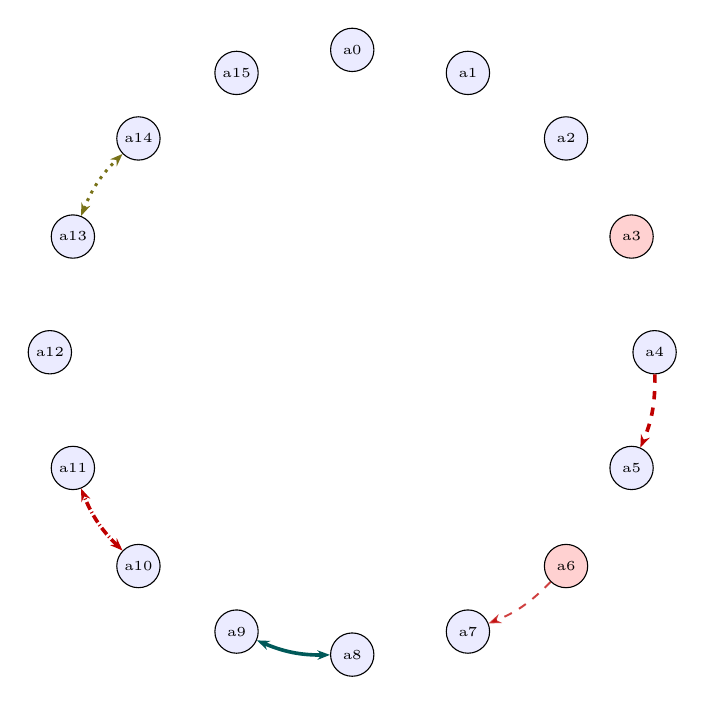
\begin{tikzpicture}[>={Stealth[length=1.6mm]}]
  \node[circle,draw,fill=blue!8,inner sep=1pt,minimum size=5.5mm,font=\tiny] (a0) at (90.0:3.84) {a0};
  \node[circle,draw,fill=blue!8,inner sep=1pt,minimum size=5.5mm,font=\tiny] (a1) at (67.5:3.84) {a1};
  \node[circle,draw,fill=blue!8,inner sep=1pt,minimum size=5.5mm,font=\tiny] (a2) at (45.0:3.84) {a2};
  \node[circle,draw,fill=red!18,inner sep=1pt,minimum size=5.5mm,font=\tiny] (a3) at (22.5:3.84) {a3};
  \node[circle,draw,fill=blue!8,inner sep=1pt,minimum size=5.5mm,font=\tiny] (a4) at (0.0:3.84) {a4};
  \node[circle,draw,fill=blue!8,inner sep=1pt,minimum size=5.5mm,font=\tiny] (a5) at (-22.5:3.84) {a5};
  \node[circle,draw,fill=red!18,inner sep=1pt,minimum size=5.5mm,font=\tiny] (a6) at (-45.0:3.84) {a6};
  \node[circle,draw,fill=blue!8,inner sep=1pt,minimum size=5.5mm,font=\tiny] (a7) at (-67.5:3.84) {a7};
  \node[circle,draw,fill=blue!8,inner sep=1pt,minimum size=5.5mm,font=\tiny] (a8) at (-90.0:3.84) {a8};
  \node[circle,draw,fill=blue!8,inner sep=1pt,minimum size=5.5mm,font=\tiny] (a9) at (-112.5:3.84) {a9};
  \node[circle,draw,fill=blue!8,inner sep=1pt,minimum size=5.5mm,font=\tiny] (a10) at (-135.0:3.84) {a10};
  \node[circle,draw,fill=blue!8,inner sep=1pt,minimum size=5.5mm,font=\tiny] (a11) at (-157.5:3.84) {a11};
  \node[circle,draw,fill=blue!8,inner sep=1pt,minimum size=5.5mm,font=\tiny] (a12) at (-180.0:3.84) {a12};
  \node[circle,draw,fill=blue!8,inner sep=1pt,minimum size=5.5mm,font=\tiny] (a13) at (-202.5:3.84) {a13};
  \node[circle,draw,fill=blue!8,inner sep=1pt,minimum size=5.5mm,font=\tiny] (a14) at (-225.0:3.84) {a14};
  \node[circle,draw,fill=blue!8,inner sep=1pt,minimum size=5.5mm,font=\tiny] (a15) at (-247.5:3.84) {a15};
  \draw[-{Stealth[length=1.6mm]}, red!75!black, dashed, line width=1.31pt] (a4) to[bend left=12] (a5);
  \draw[-{Stealth[length=1.6mm]}, red!75!black, dashed, opacity=0.75, line width=0.71pt] (a6) to[bend left=12] (a7);
  \draw[{Stealth[length=1.6mm]}-{Stealth[length=1.6mm]}, teal!70!black, line width=1.31pt] (a8) to[bend left=12] (a9);
  \draw[{Stealth[length=1.6mm]}-{Stealth[length=1.6mm]}, red!75!black, densely dashdotted, line width=1.31pt] (a10) to[bend left=12] (a11);
  \draw[{Stealth[length=1.6mm]}-{Stealth[length=1.6mm]}, olive!80!black, dotted, line width=1.08pt] (a13) to[bend left=12] (a14);
\end{tikzpicture}
}
\\[2pt]{\footnotesize valid edges only: 5 factors}
\end{minipage}
\caption{Relation graph for \texttt{locobench-claude-5-fixed-f001-r1}. Nodes are atoms on a circle, tinted red when the item marks them non-factual (prior 0.1) and blue when factual (prior 0.9). Edges are gold relations: solid blue = entailment, dashed red = contradiction, double-headed teal = equivalence, dash-dotted red (double-headed) = exclusive (exactly-one), dotted olive (double-headed) = co-necessity (at-least-one); thickness scales with the factor probability. Ordering-only Precedence edges carry no factor and so are not drawn.}
\label{fig:graph-locobench-claude-5-fixed-f001-r1}
\end{figure}

\begin{table}[htbp]
\centering
\footnotesize
\setlength{\tabcolsep}{3.5pt}
\caption{The specific gold relations of \texttt{locobench-claude-5-fixed-f001-r1}. \textbf{$p$ used} is the factor probability the MRF received: the band midpoint, times $(1-\lambda)$ for a resolved concession, or \emph{none} for an ordering-only edge (no factor). \textbf{Valid} marks the deliberately-planted errors with their kind. \textbf{Res.} is the resolving atom of a resolved concession.}
\label{tab:rels-locobench-claude-5-fixed-f001-r1}
\begin{tabular}{lllllrll}
\toprule
ID & Endpoints & Sense & Coupling & Band & $p$ used & Valid & Res. \\
\midrule
\texttt{r000} & \texttt{a0} $\to$ \texttt{a1} & Precedence & \texttt{none} & moderate & \emph{none} & \checkmark &  \\
\texttt{r001} & \texttt{a2} $\to$ \texttt{a5} & Effect-Cause & \texttt{entailment} & moderate & 0.720 & $\times$ {\scriptsize wrong\_direction} &  \\
\texttt{r002} & \texttt{a3} $\leftrightarrow$ \texttt{a2} & Contrast & \texttt{contradiction} & weak & 0.470 & $\times$ {\scriptsize false\_endpoint} &  \\
\texttt{r003} & \texttt{a4} $\leftrightarrow$ \texttt{a5} & Contrast & \texttt{contradiction} & strong & 0.925 & \checkmark &  \\
\texttt{r004} & \texttt{a6} $\to$ \texttt{a7} & Concession & \texttt{contradiction} & moderate & 0.396 & \checkmark & \texttt{a12} \\
\texttt{r005} & \texttt{a8} $\to$ \texttt{a7} & Evidence & \texttt{entailment} & moderate & 0.720 & $\times$ {\scriptsize wrong\_direction} &  \\
\texttt{r006} & \texttt{a8} $\leftrightarrow$ \texttt{a9} & Restatement & \texttt{equivalence} & strong & 0.925 & \checkmark &  \\
\texttt{r007} & \texttt{a10} $\leftrightarrow$ \texttt{a11} & Alternative & \texttt{exclusive} & strong & 0.925 & \checkmark &  \\
\texttt{r008} & \texttt{a13} $\leftrightarrow$ \texttt{a14} & Disjunction & \texttt{co\_necessity} & moderate & 0.720 & \checkmark &  \\
\texttt{r009} & \texttt{a15} $\to$ \texttt{a14} & Cause-Effect & \texttt{entailment} & weak & 0.470 & $\times$ {\scriptsize spurious} &  \\
\bottomrule
\end{tabular}
\end{table}

\begin{table}[htbp]
\centering
\footnotesize
\caption{Atoms of \texttt{locobench-claude-5-fixed-f001-r1}: the \texttt{factual} label, the prior it maps to, the posterior marginal $P(a_i{=}1)$ the MRF returns, and the shift. Atoms dragged below their prior are the ones the coherence structure penalises.}
\label{tab:atoms-locobench-claude-5-fixed-f001-r1}
\begin{tabular}{llrrrp{7.2cm}}
\toprule
Atom & fact & $\pi_i$ & $P(a_i{=}1)$ & $\Delta$ & Text \\
\midrule
\texttt{a0} & \checkmark & 0.90 & 0.900 & +0.000 & \footnotesize Excavators record the position and orientation of each bone in situ before the remains are lifted. \\
\texttt{a1} & \checkmark & 0.90 & 0.900 & +0.000 & \footnotesize Several independent osteologists score the same lesions to test inter-observer reliability. \\
\texttt{a2} & \checkmark & 0.90 & 0.904 & +0.004 & \footnotesize The loss of collagen after death shifts the bone's response to loading from plastic to brittle. \\
\texttt{a3} & $\times$ & 0.10 & 0.104 & +0.004 & \footnotesize Buried bone retains its fresh, plastic mechanical properties for approximately fifty years after death. \\
\texttt{a4} & \checkmark & 0.90 & 0.672 & -0.228 & \footnotesize Perimortem fractures in fresh bone produce beveled or obliquely angled fracture margins. \\
\texttt{a5} & \checkmark & 0.90 & 0.735 & -0.165 & \footnotesize Postmortem breaks in dry bone typically show transverse edges meeting the cortical surface at right angles. \\
\texttt{a6} & $\times$ & 0.10 & 0.117 & +0.017 & \footnotesize Postmortem dry-bone fractures produce beveled margins with adhering flakes of cortical bone. \\
\texttt{a7} & \checkmark & 0.90 & 0.959 & +0.059 & \footnotesize Adhering bone flakes and hinge fractures indicate the bone was fresh when it broke. \\
\texttt{a8} & \checkmark & 0.90 & 0.985 & +0.085 & \footnotesize The fracture occurred while the bone was still fresh and elastic. \\
\texttt{a9} & \checkmark & 0.90 & 0.982 & +0.082 & \footnotesize The break happened at or near the time of death, before the bone's collagen degraded. \\
\texttt{a10} & \checkmark & 0.90 & 0.632 & -0.268 & \footnotesize Every fracture margin on the skeleton was produced after death. \\
\texttt{a11} & \checkmark & 0.90 & 0.632 & -0.268 & \footnotesize At least one fracture margin on the skeleton was produced at or around the time of death. \\
\texttt{a12} & \checkmark & 0.90 & 0.900 & +0.000 & \footnotesize The review panel ultimately held that beveled fracture margins on the cranium reflect perimortem breakage. \\
\texttt{a13} & \checkmark & 0.90 & 0.929 & +0.029 & \footnotesize Scavenging animals disturbed the remains within the grave. \\
\texttt{a14} & \checkmark & 0.90 & 0.922 & +0.022 & \footnotesize Sediment loading fractured the bones after burial. \\
\texttt{a15} & \checkmark & 0.90 & 0.895 & -0.005 & \footnotesize Damage inflicted by trowels and picks during excavation can mimic ancient trauma. \\
\bottomrule
\end{tabular}
\end{table}

\subsection{Archaeology -- base (\texttt{locobench-claude-5-fixed-f002-r1})}

\textbf{Topic:} Archaeology (Humanities). \textbf{Family:} \texttt{f002} (CONFLICT), rung 1 (\emph{base}). \textbf{Scores:} mean-marg $= 0.792$, consist $= 0.075$, reified $= 0.250$, log-Z $= 0.327$.



\paragraph{Framing question.} \emph{How do archaeologists adjudicate between competing interpretations when a stratified deposit yields artifacts that appear older than the layer containing them?}



\paragraph{Response.} {\small When a stratified deposit yields material that appears to predate the layer holding it, the first task is not to discard either observation but to specify what each rests on. The law of superposition holds that in an undisturbed sequence lower deposits were laid down before those above them, and it was on the strength of that principle that the artifacts proved older than the sediment enclosing them. Chronological information at a site is carried in two partly independent registers — the order of the deposits and the age of the objects within them — and when those registers disagree the disagreement is informative rather than fatal. The same discrepancy can be stated from the other end without any change in content: equivalently, the sediment enclosing the artifacts was younger than the artifacts. What remains to be settled is which of the several histories capable of producing such an arrangement actually did so.

Two families of process can place old objects in young sediment, and they are not mutually exclusive, so at least one of the following obtained, perhaps both: older material was incorporated into the layer while the layer was forming, or older artifacts moved into the layer after the layer had formed. Discriminating between them requires a prior judgment about the integrity of the deposit, and there the options are exhaustive and mutually exclusive: either the deposit containing the artifacts was stratigraphically intact, or it was disturbed after its formation, and since both cannot be true, one of them must hold. That burrowing animals can transport artifacts vertically between stratigraphic layers indicates the second of those alternatives, post-depositional disturbance, wherever traces of such activity can be recognized in section. By contrast with that burrowing transport, bioturbation displaces artifacts downward only.

General mechanisms, however, license possibilities rather than conclusions; adjudication is achieved by site-specific argument, marshalled from the excavated record itself. Here the final excavation report concluded that the deposit had been disturbed by rodent burrowing after its formation, and that determination constitutes the strongest evidence that the deposit's stratigraphic integrity had in fact been compromised. Refitting fragments of a single broken artifact across two layers demonstrates vertical displacement of material, and that demonstration was accomplished earlier than the conclusion eventually recorded in the report, so the argument for movement between strata was already in hand when the disturbance was formally diagnosed.

Independent chronometry supplies a second line of control on the same question. Radiocarbon dating of short-lived plant remains from a context provides an age estimate for that context's formation, because seeds, twigs and other ephemeral tissues enter a deposit close to the moment it accumulates and cannot have been curated for generations beforehand. Radiocarbon dating directly measures the age at which a flint tool was knapped; the plant-based estimate, by contrast, speaks to the accumulation of the enclosing matrix rather than to the objects recovered from within it, and the two therefore answer different questions about the same anomaly.

Where rival readings survive these stratigraphic and chronometric controls, resolution becomes a matter of specialist review. Although the excavator interpreted the older flint blades as heirlooms curated by the occupants of the layer, a lithics specialist interpreted those same blades as residual material eroded from an earlier deposit, reading their condition and technological character as products of reworking rather than of deliberate retention. The impasse was closed when a review panel determined that the older flint blades were residual finds rather than curated heirlooms, a finding that removed the curation hypothesis from consideration and aligned the artifact assemblage with the depositional history reconstructed from the section. Adjudication, in short, proceeds by converting an apparent contradiction into a testable choice among formation processes, and then by letting stratigraphic observation, refitting, dating and peer scrutiny narrow that choice to one.}

\begin{figure}[htbp]
\centering
\begin{minipage}[t]{0.48\linewidth}\centering
\resizebox{!}{6.4cm}{%
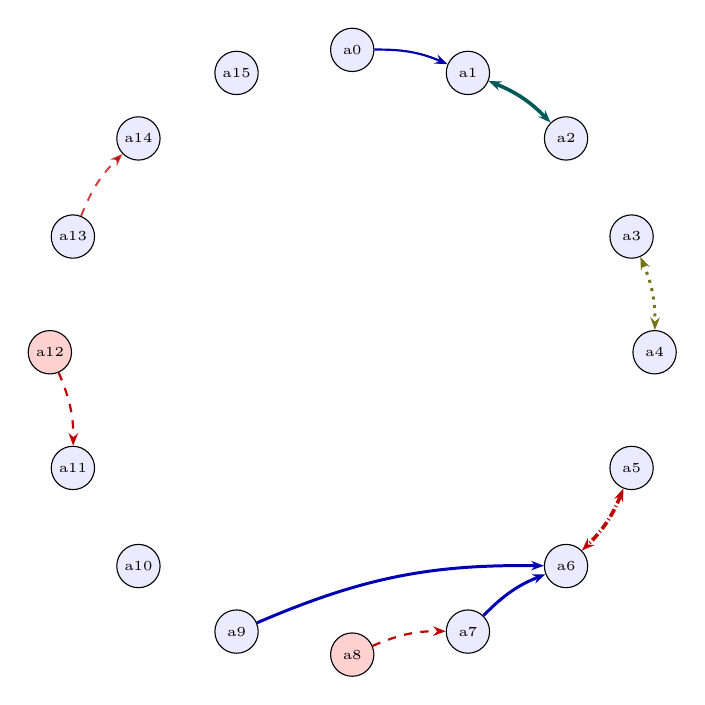
\begin{tikzpicture}[>={Stealth[length=1.6mm]}]
  \node[circle,draw,fill=blue!8,inner sep=1pt,minimum size=5.5mm,font=\tiny] (a0) at (90.0:3.84) {a0};
  \node[circle,draw,fill=blue!8,inner sep=1pt,minimum size=5.5mm,font=\tiny] (a1) at (67.5:3.84) {a1};
  \node[circle,draw,fill=blue!8,inner sep=1pt,minimum size=5.5mm,font=\tiny] (a2) at (45.0:3.84) {a2};
  \node[circle,draw,fill=blue!8,inner sep=1pt,minimum size=5.5mm,font=\tiny] (a3) at (22.5:3.84) {a3};
  \node[circle,draw,fill=blue!8,inner sep=1pt,minimum size=5.5mm,font=\tiny] (a4) at (0.0:3.84) {a4};
  \node[circle,draw,fill=blue!8,inner sep=1pt,minimum size=5.5mm,font=\tiny] (a5) at (-22.5:3.84) {a5};
  \node[circle,draw,fill=blue!8,inner sep=1pt,minimum size=5.5mm,font=\tiny] (a6) at (-45.0:3.84) {a6};
  \node[circle,draw,fill=blue!8,inner sep=1pt,minimum size=5.5mm,font=\tiny] (a7) at (-67.5:3.84) {a7};
  \node[circle,draw,fill=red!18,inner sep=1pt,minimum size=5.5mm,font=\tiny] (a8) at (-90.0:3.84) {a8};
  \node[circle,draw,fill=blue!8,inner sep=1pt,minimum size=5.5mm,font=\tiny] (a9) at (-112.5:3.84) {a9};
  \node[circle,draw,fill=blue!8,inner sep=1pt,minimum size=5.5mm,font=\tiny] (a10) at (-135.0:3.84) {a10};
  \node[circle,draw,fill=blue!8,inner sep=1pt,minimum size=5.5mm,font=\tiny] (a11) at (-157.5:3.84) {a11};
  \node[circle,draw,fill=red!18,inner sep=1pt,minimum size=5.5mm,font=\tiny] (a12) at (-180.0:3.84) {a12};
  \node[circle,draw,fill=blue!8,inner sep=1pt,minimum size=5.5mm,font=\tiny] (a13) at (-202.5:3.84) {a13};
  \node[circle,draw,fill=blue!8,inner sep=1pt,minimum size=5.5mm,font=\tiny] (a14) at (-225.0:3.84) {a14};
  \node[circle,draw,fill=blue!8,inner sep=1pt,minimum size=5.5mm,font=\tiny] (a15) at (-247.5:3.84) {a15};
  \draw[-{Stealth[length=1.6mm]}, blue!70!black, line width=0.79pt] (a0) to[bend left=12] (a1);
  \draw[{Stealth[length=1.6mm]}-{Stealth[length=1.6mm]}, teal!70!black, line width=1.31pt] (a1) to[bend left=12] (a2);
  \draw[{Stealth[length=1.6mm]}-{Stealth[length=1.6mm]}, olive!80!black, dotted, line width=1.08pt] (a3) to[bend left=12] (a4);
  \draw[{Stealth[length=1.6mm]}-{Stealth[length=1.6mm]}, red!75!black, densely dashdotted, line width=1.31pt] (a5) to[bend left=12] (a6);
  \draw[-{Stealth[length=1.6mm]}, blue!70!black, line width=1.08pt] (a7) to[bend left=12] (a6);
  \draw[-{Stealth[length=1.6mm]}, red!75!black, dashed, line width=0.79pt] (a8) to[bend left=12] (a7);
  \draw[-{Stealth[length=1.6mm]}, blue!70!black, line width=1.08pt] (a9) to[bend left=12] (a6);
  \draw[-{Stealth[length=1.6mm]}, red!75!black, dashed, line width=0.79pt] (a12) to[bend left=12] (a11);
  \draw[-{Stealth[length=1.6mm]}, red!75!black, dashed, opacity=0.75, line width=0.71pt] (a13) to[bend left=12] (a14);
\end{tikzpicture}
}
\\[2pt]{\footnotesize all gold edges: 9 factors}
\end{minipage}\hfill\begin{minipage}[t]{0.48\linewidth}\centering
\resizebox{!}{6.4cm}{%
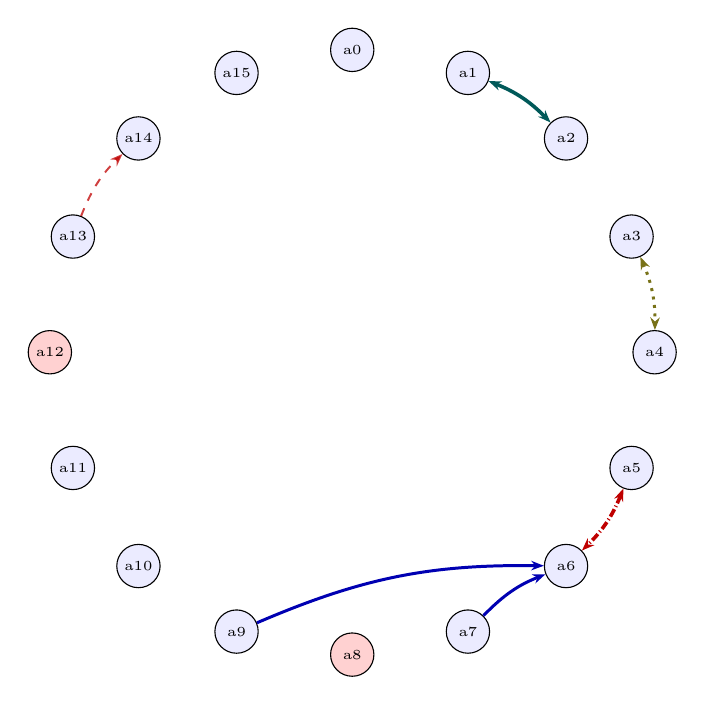
\begin{tikzpicture}[>={Stealth[length=1.6mm]}]
  \node[circle,draw,fill=blue!8,inner sep=1pt,minimum size=5.5mm,font=\tiny] (a0) at (90.0:3.84) {a0};
  \node[circle,draw,fill=blue!8,inner sep=1pt,minimum size=5.5mm,font=\tiny] (a1) at (67.5:3.84) {a1};
  \node[circle,draw,fill=blue!8,inner sep=1pt,minimum size=5.5mm,font=\tiny] (a2) at (45.0:3.84) {a2};
  \node[circle,draw,fill=blue!8,inner sep=1pt,minimum size=5.5mm,font=\tiny] (a3) at (22.5:3.84) {a3};
  \node[circle,draw,fill=blue!8,inner sep=1pt,minimum size=5.5mm,font=\tiny] (a4) at (0.0:3.84) {a4};
  \node[circle,draw,fill=blue!8,inner sep=1pt,minimum size=5.5mm,font=\tiny] (a5) at (-22.5:3.84) {a5};
  \node[circle,draw,fill=blue!8,inner sep=1pt,minimum size=5.5mm,font=\tiny] (a6) at (-45.0:3.84) {a6};
  \node[circle,draw,fill=blue!8,inner sep=1pt,minimum size=5.5mm,font=\tiny] (a7) at (-67.5:3.84) {a7};
  \node[circle,draw,fill=red!18,inner sep=1pt,minimum size=5.5mm,font=\tiny] (a8) at (-90.0:3.84) {a8};
  \node[circle,draw,fill=blue!8,inner sep=1pt,minimum size=5.5mm,font=\tiny] (a9) at (-112.5:3.84) {a9};
  \node[circle,draw,fill=blue!8,inner sep=1pt,minimum size=5.5mm,font=\tiny] (a10) at (-135.0:3.84) {a10};
  \node[circle,draw,fill=blue!8,inner sep=1pt,minimum size=5.5mm,font=\tiny] (a11) at (-157.5:3.84) {a11};
  \node[circle,draw,fill=red!18,inner sep=1pt,minimum size=5.5mm,font=\tiny] (a12) at (-180.0:3.84) {a12};
  \node[circle,draw,fill=blue!8,inner sep=1pt,minimum size=5.5mm,font=\tiny] (a13) at (-202.5:3.84) {a13};
  \node[circle,draw,fill=blue!8,inner sep=1pt,minimum size=5.5mm,font=\tiny] (a14) at (-225.0:3.84) {a14};
  \node[circle,draw,fill=blue!8,inner sep=1pt,minimum size=5.5mm,font=\tiny] (a15) at (-247.5:3.84) {a15};
  \draw[{Stealth[length=1.6mm]}-{Stealth[length=1.6mm]}, teal!70!black, line width=1.31pt] (a1) to[bend left=12] (a2);
  \draw[{Stealth[length=1.6mm]}-{Stealth[length=1.6mm]}, olive!80!black, dotted, line width=1.08pt] (a3) to[bend left=12] (a4);
  \draw[{Stealth[length=1.6mm]}-{Stealth[length=1.6mm]}, red!75!black, densely dashdotted, line width=1.31pt] (a5) to[bend left=12] (a6);
  \draw[-{Stealth[length=1.6mm]}, blue!70!black, line width=1.08pt] (a7) to[bend left=12] (a6);
  \draw[-{Stealth[length=1.6mm]}, blue!70!black, line width=1.08pt] (a9) to[bend left=12] (a6);
  \draw[-{Stealth[length=1.6mm]}, red!75!black, dashed, opacity=0.75, line width=0.71pt] (a13) to[bend left=12] (a14);
\end{tikzpicture}
}
\\[2pt]{\footnotesize valid edges only: 6 factors}
\end{minipage}
\caption{Relation graph for \texttt{locobench-claude-5-fixed-f002-r1}. Nodes are atoms on a circle, tinted red when the item marks them non-factual (prior 0.1) and blue when factual (prior 0.9). Edges are gold relations: solid blue = entailment, dashed red = contradiction, double-headed teal = equivalence, dash-dotted red (double-headed) = exclusive (exactly-one), dotted olive (double-headed) = co-necessity (at-least-one); thickness scales with the factor probability. Ordering-only Precedence edges carry no factor and so are not drawn.}
\label{fig:graph-locobench-claude-5-fixed-f002-r1}
\end{figure}

\begin{table}[htbp]
\centering
\footnotesize
\setlength{\tabcolsep}{3.5pt}
\caption{The specific gold relations of \texttt{locobench-claude-5-fixed-f002-r1}. \textbf{$p$ used} is the factor probability the MRF received: the band midpoint, times $(1-\lambda)$ for a resolved concession, or \emph{none} for an ordering-only edge (no factor). \textbf{Valid} marks the deliberately-planted errors with their kind. \textbf{Res.} is the resolving atom of a resolved concession.}
\label{tab:rels-locobench-claude-5-fixed-f002-r1}
\begin{tabular}{lllllrll}
\toprule
ID & Endpoints & Sense & Coupling & Band & $p$ used & Valid & Res. \\
\midrule
\texttt{r000} & \texttt{a0} $\to$ \texttt{a1} & Cause-Effect & \texttt{entailment} & weak & 0.470 & $\times$ {\scriptsize spurious} &  \\
\texttt{r001} & \texttt{a1} $\leftrightarrow$ \texttt{a2} & Restatement & \texttt{equivalence} & strong & 0.925 & \checkmark &  \\
\texttt{r002} & \texttt{a3} $\leftrightarrow$ \texttt{a4} & Disjunction & \texttt{co\_necessity} & moderate & 0.720 & \checkmark &  \\
\texttt{r003} & \texttt{a5} $\leftrightarrow$ \texttt{a6} & Alternative & \texttt{exclusive} & strong & 0.925 & \checkmark &  \\
\texttt{r004} & \texttt{a7} $\to$ \texttt{a6} & Evidence & \texttt{entailment} & moderate & 0.720 & \checkmark &  \\
\texttt{r005} & \texttt{a8} $\leftrightarrow$ \texttt{a7} & Contrast & \texttt{contradiction} & weak & 0.470 & $\times$ {\scriptsize false\_endpoint} &  \\
\texttt{r006} & \texttt{a9} $\to$ \texttt{a6} & Evidence & \texttt{entailment} & moderate & 0.720 & \checkmark &  \\
\texttt{r007} & \texttt{a10} $\to$ \texttt{a9} & Precedence & \texttt{none} & weak & \emph{none} & $\times$ {\scriptsize wrong\_sense} &  \\
\texttt{r008} & \texttt{a12} $\leftrightarrow$ \texttt{a11} & Contrast & \texttt{contradiction} & weak & 0.470 & $\times$ {\scriptsize false\_endpoint} &  \\
\texttt{r009} & \texttt{a13} $\to$ \texttt{a14} & Concession & \texttt{contradiction} & moderate & 0.396 & \checkmark & \texttt{a15} \\
\bottomrule
\end{tabular}
\end{table}

\begin{table}[htbp]
\centering
\footnotesize
\caption{Atoms of \texttt{locobench-claude-5-fixed-f002-r1}: the \texttt{factual} label, the prior it maps to, the posterior marginal $P(a_i{=}1)$ the MRF returns, and the shift. Atoms dragged below their prior are the ones the coherence structure penalises.}
\label{tab:atoms-locobench-claude-5-fixed-f002-r1}
\begin{tabular}{llrrrp{7.2cm}}
\toprule
Atom & fact & $\pi_i$ & $P(a_i{=}1)$ & $\Delta$ & Text \\
\midrule
\texttt{a0} & \checkmark & 0.90 & 0.895 & -0.005 & \footnotesize The law of superposition holds that in an undisturbed sequence lower deposits were laid down before those above them. \\
\texttt{a1} & \checkmark & 0.90 & 0.977 & +0.077 & \footnotesize The artifacts were older than the sediment that enclosed them. \\
\texttt{a2} & \checkmark & 0.90 & 0.978 & +0.078 & \footnotesize The sediment enclosing the artifacts was younger than the artifacts. \\
\texttt{a3} & \checkmark & 0.90 & 0.929 & +0.029 & \footnotesize Older material was incorporated into the layer while the layer was forming. \\
\texttt{a4} & \checkmark & 0.90 & 0.929 & +0.029 & \footnotesize Older artifacts moved into the layer after the layer had formed. \\
\texttt{a5} & \checkmark & 0.90 & 0.478 & -0.422 & \footnotesize The deposit containing the artifacts was stratigraphically intact. \\
\texttt{a6} & \checkmark & 0.90 & 0.902 & +0.002 & \footnotesize The deposit containing the artifacts was disturbed after its formation. \\
\texttt{a7} & \checkmark & 0.90 & 0.920 & +0.020 & \footnotesize Burrowing animals can transport artifacts vertically between stratigraphic layers. \\
\texttt{a8} & $\times$ & 0.10 & 0.105 & +0.005 & \footnotesize Bioturbation displaces artifacts downward only. \\
\texttt{a9} & \checkmark & 0.90 & 0.919 & +0.019 & \footnotesize The final excavation report concluded that the deposit had been disturbed by rodent burrowing after its formation. \\
\texttt{a10} & \checkmark & 0.90 & 0.900 & +0.000 & \footnotesize Refitting fragments of a single broken artifact across two layers demonstrates vertical displacement of material. \\
\texttt{a11} & \checkmark & 0.90 & 0.901 & +0.001 & \footnotesize Radiocarbon dating of short-lived plant remains from a context provides an age estimate for that context's formation. \\
\texttt{a12} & $\times$ & 0.10 & 0.104 & +0.004 & \footnotesize Radiocarbon dating directly measures the age at which a flint tool was knapped. \\
\texttt{a13} & \checkmark & 0.90 & 0.913 & +0.013 & \footnotesize The excavator interpreted the older flint blades as heirlooms curated by the occupants of the layer. \\
\texttt{a14} & \checkmark & 0.90 & 0.929 & +0.029 & \footnotesize A lithics specialist interpreted the older flint blades as residual material eroded from an earlier deposit. \\
\texttt{a15} & \checkmark & 0.90 & 0.900 & +0.000 & \footnotesize A review panel determined that the older flint blades were residual finds rather than curated heirlooms. \\
\bottomrule
\end{tabular}
\end{table}

\section{Findings}

\begin{itemize}
\item \textbf{Every rung carries its own gold relations, so the ladder is a real test.} On the \texttt{gold} arm 22 of 28 ordering assertions hold across all families (\texttt{consist} 7/8, \texttt{log-Z} 8/10, \texttt{mean-marg} 7/10). Because each rung's labels describe the response that ships with them, these pass rates are evidence about the readouts rather than about the corpus --- which is what the previous generation of this dataset could not provide.
\item \textbf{The readouts differ sharply in sensitivity.} Across the 10 scored items \texttt{mean\_marginal} spans only $[0.750, 0.824]$, while \texttt{consistency} spans $[0.015, 0.341]$. With atom priors pinned at $0.9/0.1$ the mean marginal is dominated by those priors and moves little; the conflict-sensitive readouts are what register the contradiction structure. For a benchmark whose families vary conflict structure, \texttt{consistency} and \texttt{log\_partition} are the discriminating readouts.
\item \textbf{The planted invalid relations carry most of the incoherence.} Dropping them changes \texttt{consistency} by 0.000 to 0.318 across items. The planted errors are largely conflict edges anchored to a false endpoint, so they add active contradictions, and the intended-correct subgraph is markedly more coherent. That the effect runs in this direction is a sanity check that the gold labels and the MRF encoding agree about which edges are the damaging ones.
\item \textbf{Relation counts and factor counts are not the same number.} Of 96 gold relations, 10 are Precedence edges that couple no truth values and never reach the MRF, and 37 are deliberately invalid. Any comparison of graph density needs both figures; Table~\ref{tab:dataset} reports them separately for that reason.
\end{itemize}

\section{Threats to validity}

\begin{itemize}
\item \textbf{Gold relations are labels, not measurements.} The factor probability is a band midpoint, so a \texttt{strong} edge enters at exactly 0.925 whatever the underlying text supports. Nothing here tests the miner's calibration: this evaluates the MRF encoding and the readouts \emph{given} perfect relation labels. Treat these scores as a reference point for a mined arm, not as a mining result.
\item \textbf{Two families is a small sample.} The dataset has 2 families over 10 items, all generated by one model. The spreads quoted above describe this dataset; no significance claim is made or implied.
\item \textbf{The ladder tests the readouts, not the miner.} Gold relations vary per rung, so the ordering constraints are a real test --- but of the MRF encoding and the readouts given perfect labels. A live system also has to \emph{recover} those relations from the text, and nothing here measures that.
\item \textbf{The concession discount is applied from the label.} Using the item's \texttt{resolver\_atom\_id} bypasses the text heuristic a live miner must use, so the resolved-concession behaviour shown here is the best case for that mechanism.
\item \textbf{Inference is approximate in general.} Merlin runs weighted mini-bucket at a finite $i$-bound. On these 16-atom networks the induced width is small enough that it reports exact inference, but the normalized log-partition also depends on a MAP floor and a contradiction-free ceiling, so it is the readout most sensitive to any approximation.
\end{itemize}

\end{document}
